\documentclass[10pt]{article}  

%%%%%%%% PREÁMBULO %%%%%%%%%%%%
\title{Plantilla para prácticas de UGR}
\usepackage[spanish]{babel} %Indica que escribiermos en español
\usepackage[utf8]{inputenc} %Indica qué codificación se está usando ISO-8859-1(latin1)  o utf8  
\usepackage{amsmath} % Comandos extras para matemáticas (cajas para ecuaciones,
% etc)
\usepackage{amssymb} % Simbolos matematicos (por lo tanto)
\usepackage{graphicx} % Incluir imágenes en LaTeX
\usepackage{color} % Para colorear texto
\usepackage{subfigure} % subfiguras
\usepackage{float} %Podemos usar el especificador [H] en las figuras para que se
% queden donde queramos
\usepackage{capt-of} % Permite usar etiquetas fuera de elementos flotantes
% (etiquetas de figuras)
\usepackage{sidecap} % Para poner el texto de las imágenes al lado
	\sidecaptionvpos{figure}{c} % Para que el texto se alinie al centro vertical
\usepackage{caption} % Para poder quitar numeracion de figuras
\usepackage{commath} % funcionalidades extras para diferenciales, integrales,
% etc (\od, \dif, etc)
\usepackage{cancel} % para cancelar expresiones (\cancelto{0}{x})

\graphicspath{{/Users/jesusgarciamanday/Desktop/Master/CC-II/Practicas/Practica5/p5/Imagenes/}}

\usepackage{anysize} 					% Para personalizar el ancho de  los márgenes
\marginsize{2cm}{2cm}{2cm}{2cm} % Izquierda, derecha, arriba, abajo

\usepackage{appendix}
\renewcommand{\appendixname}{Apéndices}
\renewcommand{\appendixtocname}{Apéndices}
\renewcommand{\appendixpagename}{Apéndices} 

% Para que las referencias sean hipervínculos a las figuras o ecuaciones y
% aparezcan en color
\usepackage[colorlinks=true,plainpages=true,citecolor=blue,linkcolor=blue]{hyperref}
%\usepackage{hyperref} 
% Para agregar encabezado y pie de página
\usepackage{fancyhdr} 
\pagestyle{fancy}
\fancyhf{}
\fancyhead[L]{\footnotesize UGR} %encabezado izquierda
\fancyhead[R]{\footnotesize CCIA}   % dereecha
\fancyfoot[R]{\footnotesize Pr\'actica 5 - Big Data }  % Pie derecha
\fancyfoot[C]{\thepage}  % centro
\fancyfoot[L]{\footnotesize Master en Ingenier\'ia Inform\'atica }  %izquierda
\renewcommand{\footrulewidth}{0.4pt}


\usepackage{listings} % Para usar código fuente
\definecolor{dkgreen}{rgb}{0,0.6,0} % Definimos colores para usar en el código
\definecolor{gray}{rgb}{0.5,0.5,0.5} 
% configuración para el lenguaje que queramos utilizar
\lstset{language=Matlab,
   keywords={break,case,catch,continue,else,elseif,end,for,function,
      global,if,otherwise,persistent,return,switch,try,while},
   basicstyle=\ttfamily,
   keywordstyle=\color{blue},
   commentstyle=\color{red},
   stringstyle=\color{dkgreen},
   numbers=left,
   numberstyle=\tiny\color{gray},
   stepnumber=1,
   numbersep=10pt,
   backgroundcolor=\color{white},
   tabsize=4,
   showspaces=false,
   showstringspaces=false}

\newcommand{\sen}{\operatorname{\sen}}	% Definimos el comando \sen para el seno
%en español

\title{Práctica 5 - Ciencia de Datos con Hadoop}

%%%%%%%% TERMINA PREÁMBULO %%%%%%%%%%%%

\begin{document}

%%%%%%%%%%%%%%%%%%%%%%%%%%%%%%%%%% PORTADA %%%%%%%%%%%%%%%%%%%%%%%%%%%%%%%%%%%%%%%%%%%%
																					%%%
\begin{center}																		%%%
\newcommand{\HRule}{\rule{\linewidth}{0.5mm}}									%%%\left
 																					%%%
\begin{minipage}{0.48\textwidth} \begin{flushleft}
%
\includegraphics[scale = 0.63]{Imagenes/logo_upiita}
\end{flushleft}\end{minipage}
\begin{minipage}{0.48\textwidth} \begin{flushright}
%
\includegraphics[scale = 0.35]{Imagenes/IPN}
\end{flushright}\end{minipage}

													 								%%%
\vspace*{-1.5cm}								%%%
																					%%%	
\textsc{\huge Universidad de\\ \vspace{5px} Granada}\\[1.5cm]	

\textsc{\LARGE Master Profesional en Ingenier\'ia Inform\'atica }\\[1.5cm]													%%%

\begin{minipage}{0.9\textwidth} 
\begin{center}																					%%%
\textsc{\LARGE Pr\'actica 4}
\end{center}
\end{minipage}\\[0.5cm]
%%%
    																				%%%
 			\vspace*{1cm}																		%%%
																					%%%
\HRule \\[0.4cm]																	%%%
{ \huge \bfseries Hadoop}\\[0.4cm]	%%%
 																					%%%
\HRule \\[1.5cm]																	%%%
 																				%%%
																					%%%
\begin{minipage}{0.46\textwidth}													%%%
\begin{flushleft} \large															%%%
\emph{Autor:}\\	
Manuel Jes\'us Garc\'ia Manday (nickter@correo.ugr.es)\\
%%%
			%\vspace*{2cm}	
            													%%%
										 						%%%
\end{flushleft}																		%%%
\end{minipage}		
																%%%
\begin{minipage}{0.52\textwidth}		
\vspace{-0.6cm}											%%%
\begin{flushright} \large															%%%
													%%%
\end{flushright}																	%%%
\end{minipage}	
\vspace*{1cm}
%\begin{flushleft}
 	
%\end{flushleft}
%%%
 		\flushleft{\textbf{\Large Master en Ingenier\'ia Inform\'atica}	}\\																		%%%
\vspace{2cm} 																				
\begin{center}																					
{\large \today}																	%%%
 			\end{center}												  						
\end{center}							 											
																					
\newpage																		
%%%%%%%%%%%%%%%%%%%% TERMINA PORTADA %%%%%%%%%%%%%%%%%%%%%%%%%%%%%%%%

\tableofcontents 

\newpage

\section{Objetivo.}
El objetivo de esta práctica es conocer las alternativas para realizar experimentaciones de Ciencia de Datos. Para ello haremos uso del entorno \textbf{Hadoop}, utilizando \textbf{HDFS} como sistema de archivos distribuido y \textbf{MapReduce} como mecanismo de ejecución. Por último, aplicaremos la biblioteca \textbf{Mahout} para lanzar algoritmos de clasificación sobre conjuntos tipo \textbf{Big Data}.


\section{Introduccíon.}
Para comenzar a realizar las tareas  que se piden en esta práctica, es necesario en primer lugar realizar una serie de pasos iniciales que se describen a continuación. \\

Realizamos una conexión remota hacía el servidor \textbf{haddop.ugr.es} y una vez dentro comprobamos la existencia del conjunto de datos en el direcctorio indicado. \\

 \begin{figure}[H]
	\begin{center}
 		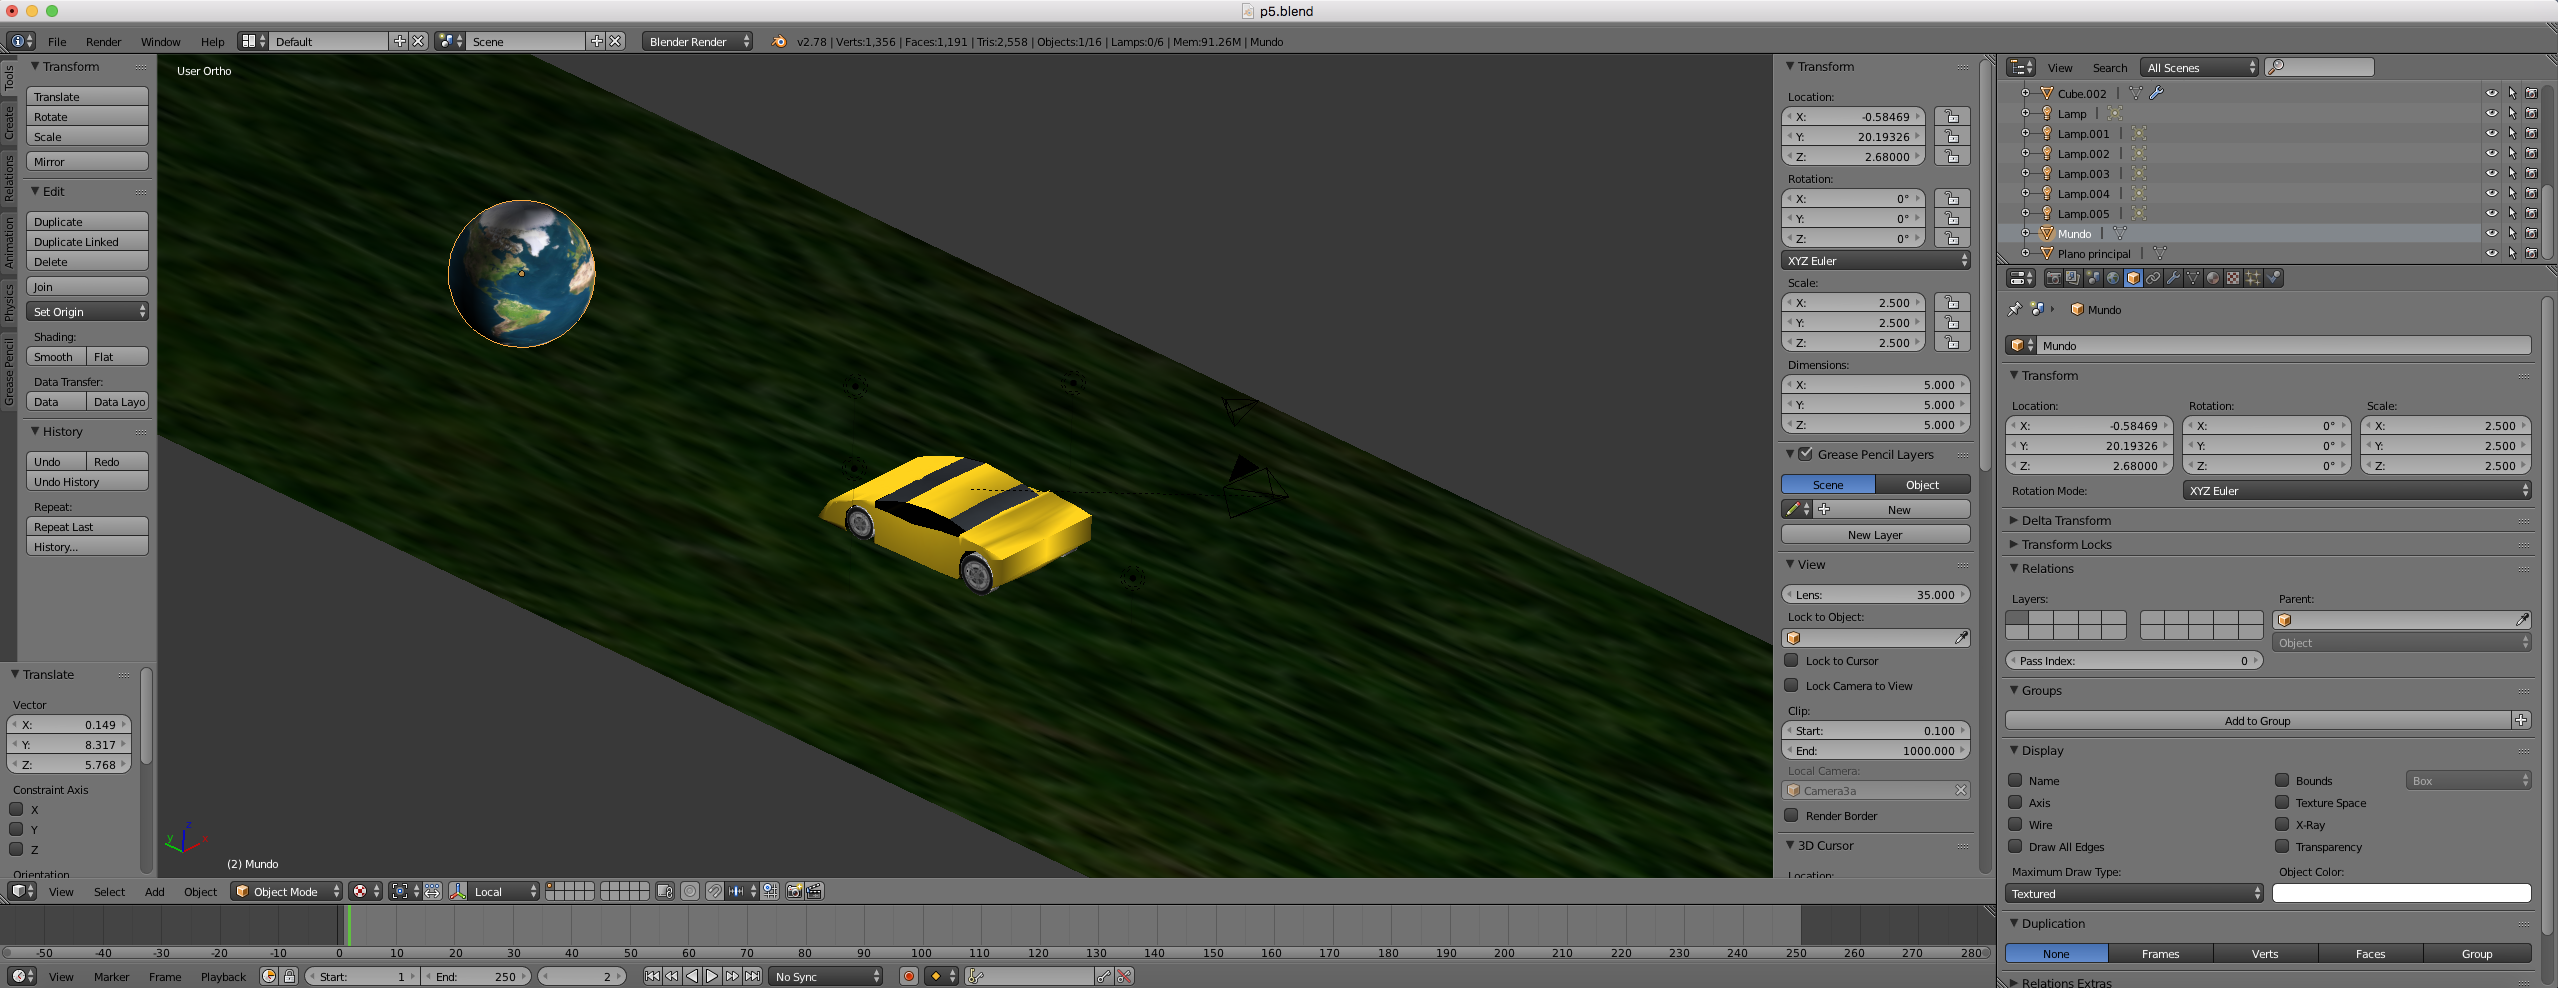
\includegraphics[width = 1.00\textwidth]{p5-img1}
 		\captionof{figure}{\label{fig:IPN}Conexion remota a \textbf{hadoop.ugr.es}.} 
	\end{center} 
\end{figure}

 \begin{figure}[H]
	\begin{center}
 		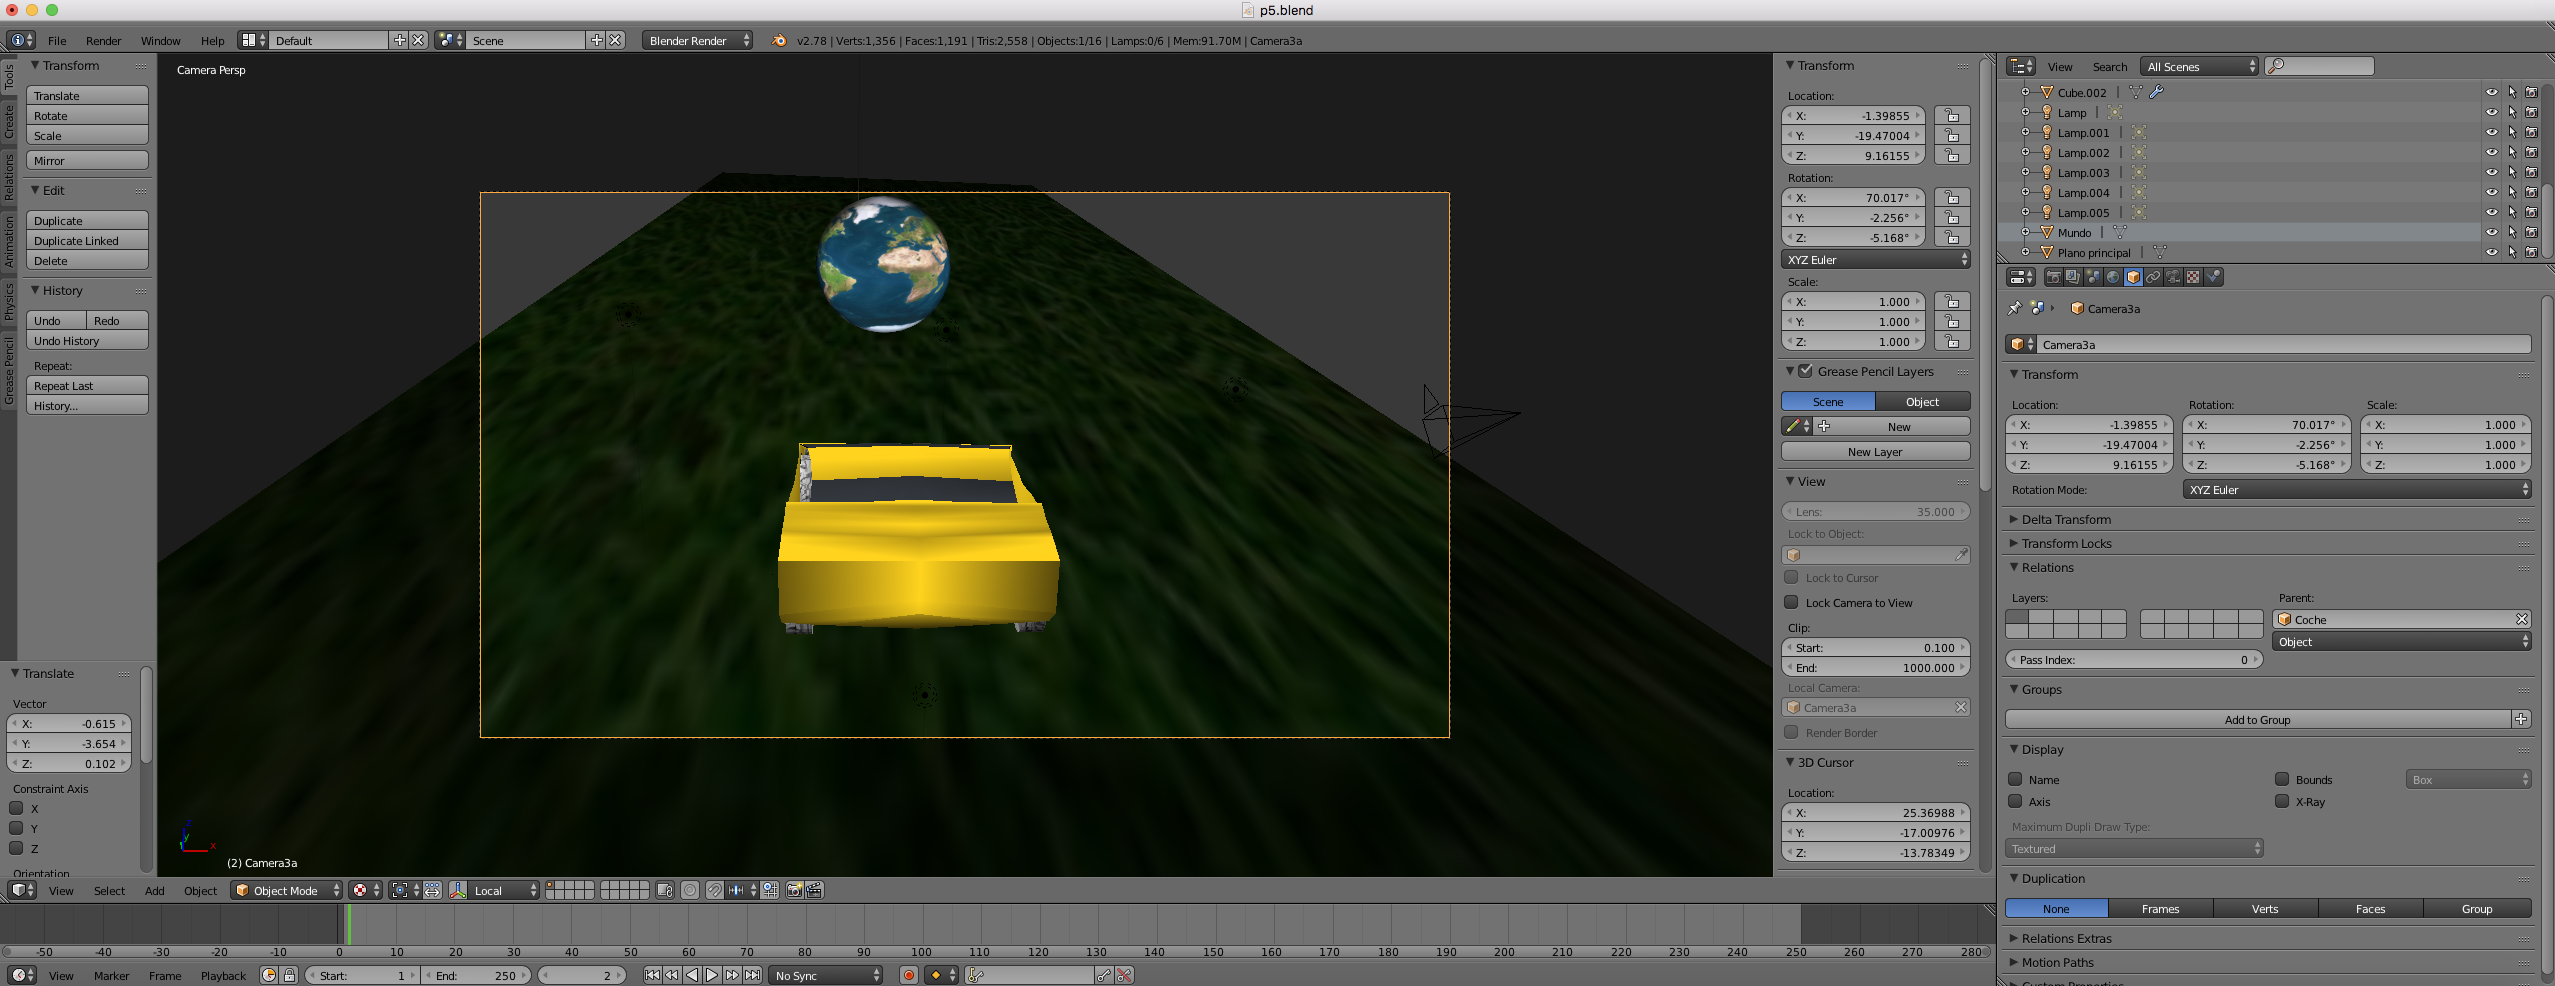
\includegraphics[width = 1.00\textwidth]{p5-img2}
 		\captionof{figure}{\label{fig:IPN}Comprobando los datasets.} 
	\end{center} 
\end{figure}


Una vez corroborada su existencia copiamos dicha carpeta en un directorio local, para posteriormente copiarla en un directorio en \textbf{hdfs} que hayamos creado previamente. \\

 \begin{figure}[H]
	\begin{center}
 		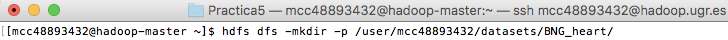
\includegraphics[width = 1.00\textwidth]{p5-img3}
 		\captionof{figure}{\label{fig:IPN}Creando nuevo directorio en \textbf{hdfs}.} 
	\end{center} 
\end{figure}

 \begin{figure}[H]
	\begin{center}
 		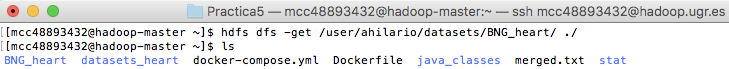
\includegraphics[width = 1.00\textwidth]{p5-img4}
 		\captionof{figure}{\label{fig:IPN}Trayendo datasets en un directorio local.} 
	\end{center} 
\end{figure}

 \begin{figure}[H]
	\begin{center}
 		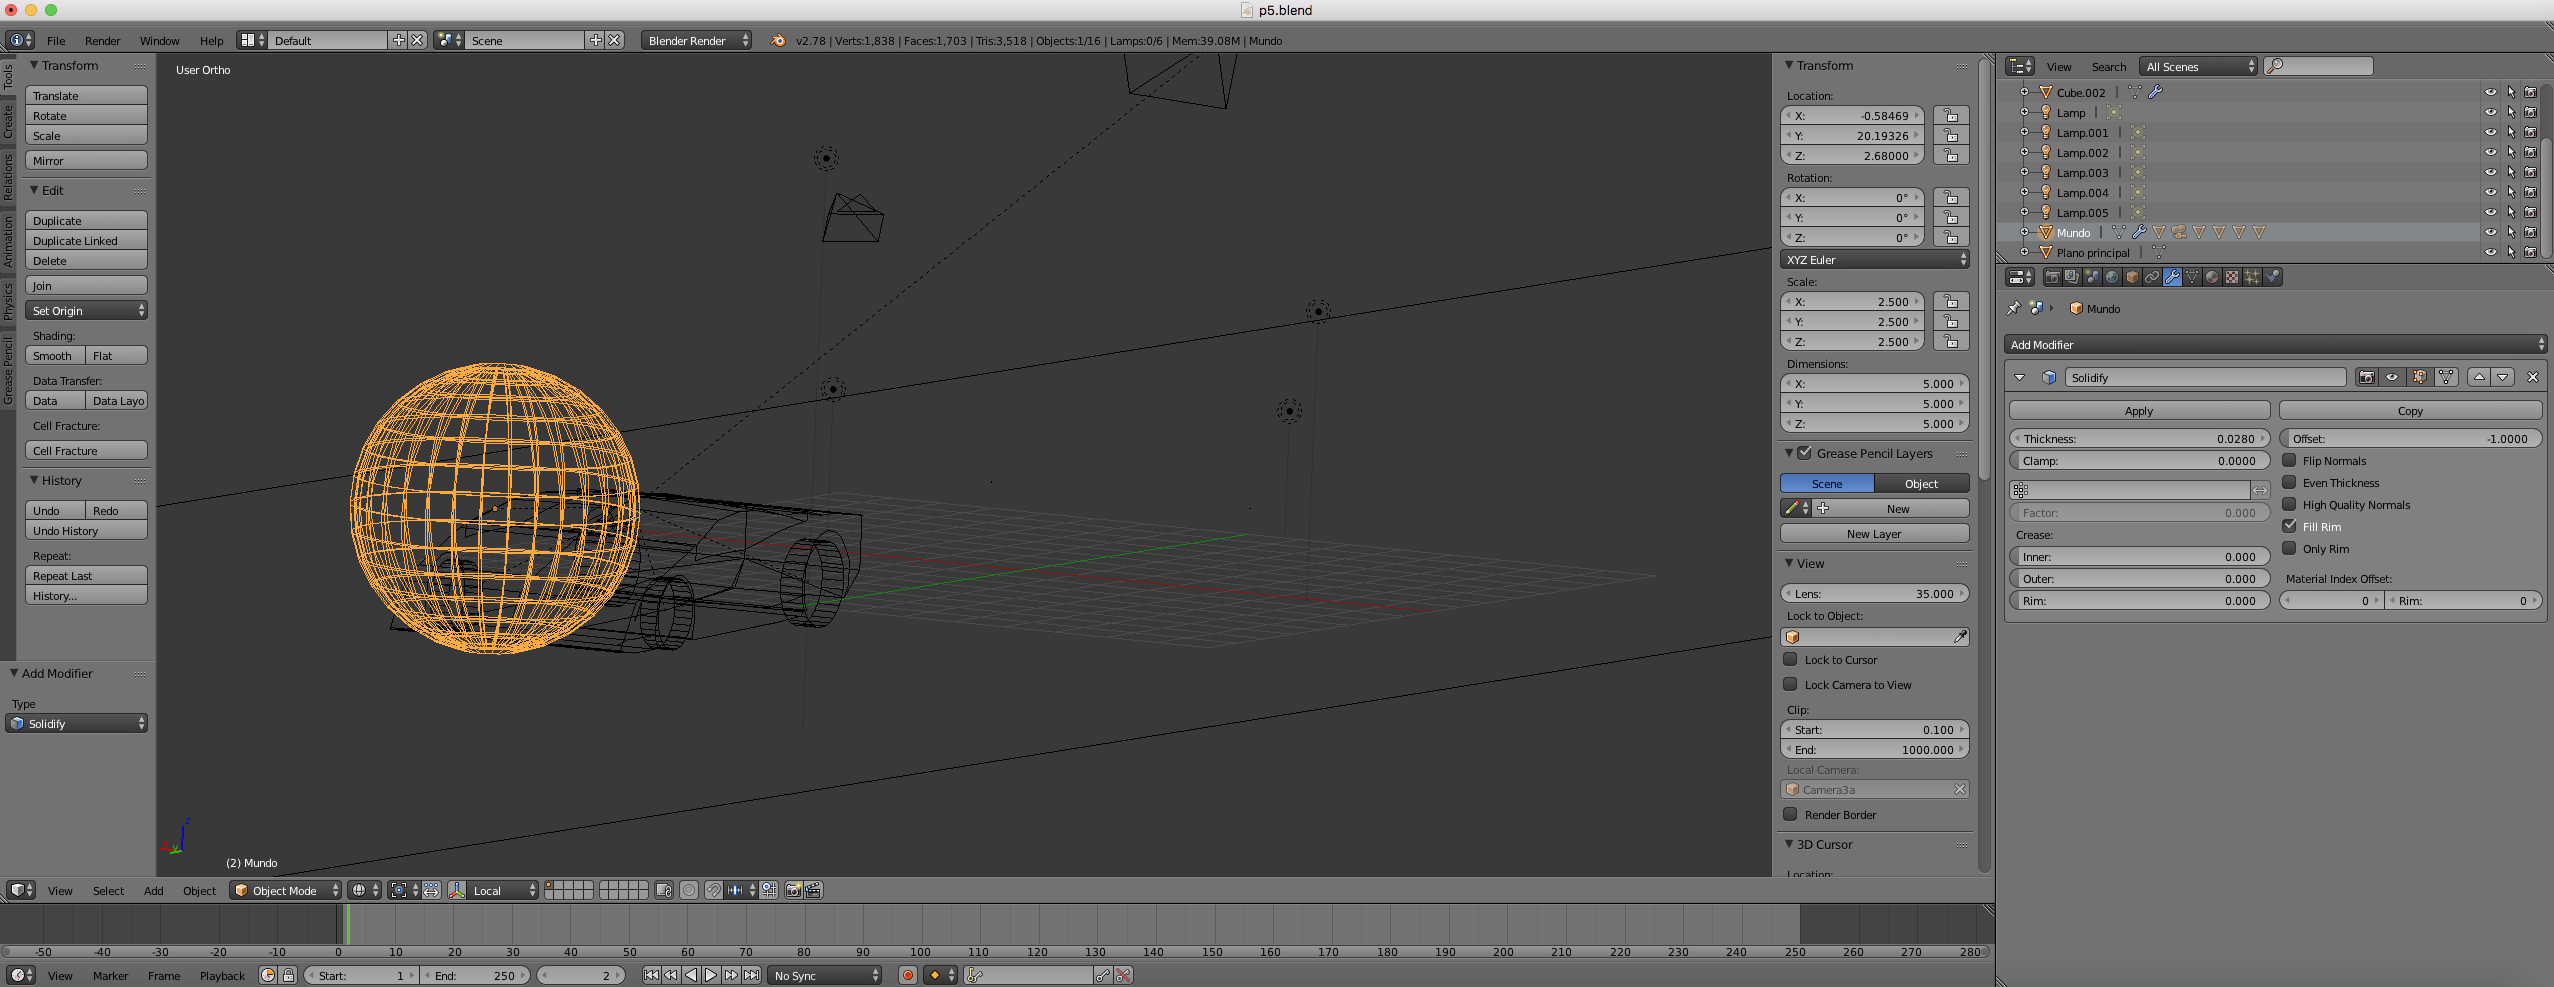
\includegraphics[width = 1.00\textwidth]{p5-img5}
 		\captionof{figure}{\label{fig:IPN}Importando datasets a un directorio \textbf{hdfs}.} 
	\end{center} 
\end{figure}

\section{Tareas.}
\subsection{Ejecutar el algoritmo ''Random Forest'' sobre el conjunto de datos BNG\_heart y comprobar el rendimiento alcanzado de acuerdo a los siguientes casos.}
Con los datasets importados a nuestro directorio de usuario en \textbf{hdfs} vamos ahora a proceder a indicar el tamaño de los datos para la partición de entrenamiento \textbf{BNG\_heart-5-1tra.dat} así como también generar los descriptores del conjunto de datos que son necesarios para la ejecución de los métodos. \\

 \begin{figure}[H]
	\begin{center}
 		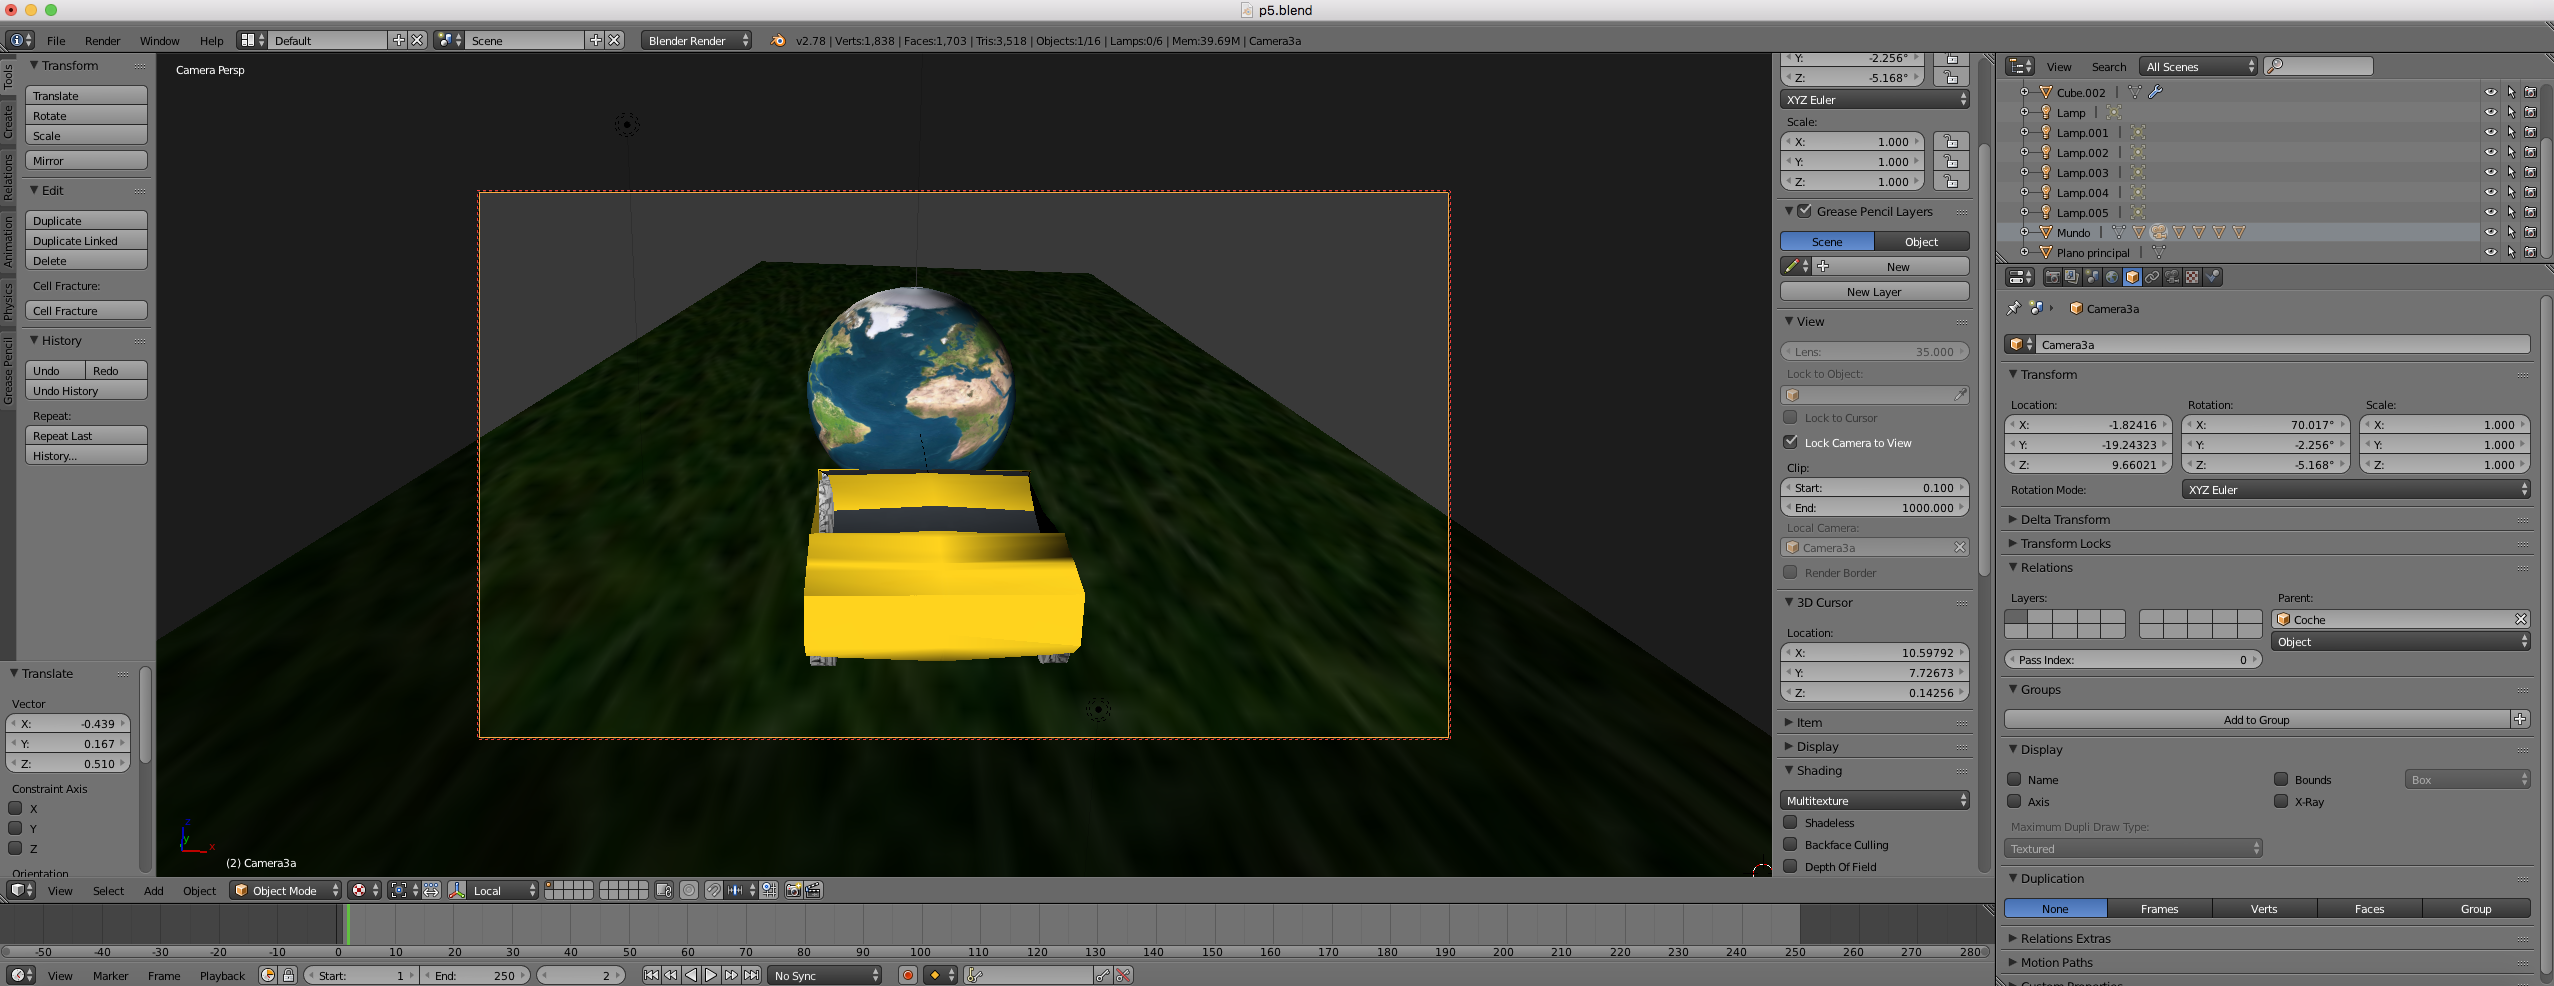
\includegraphics[width = 1.00\textwidth]{p5-img6}
 		\captionof{figure}{\label{fig:IPN}Obteniendo tamaño y generando descriptores para el conjunto de datos.} 
	\end{center} 
\end{figure}


 

\end{document}